		\documentclass[12pt]{standalone}
\usepackage{tikz}
\usetikzlibrary{calc, arrows.meta}
\begin{document}
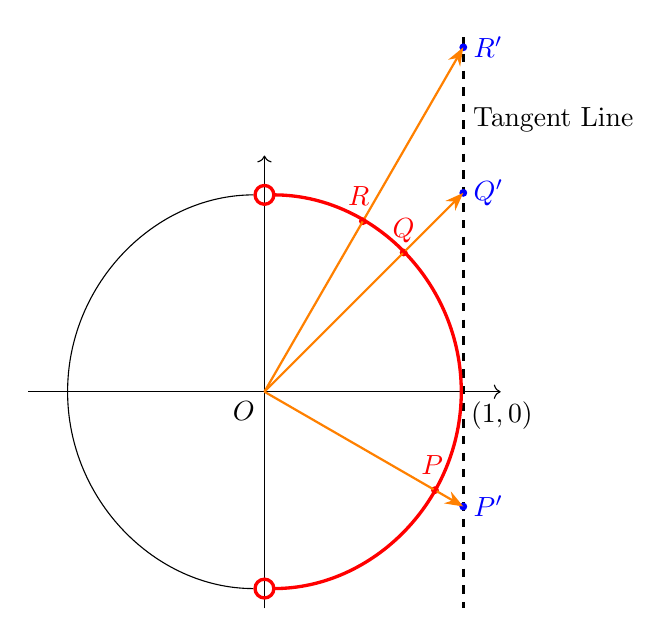
\begin{tikzpicture}[scale=2.5]
			% Define the points O and T (the origin and the tangent point)
			\coordinate (O) at (0, 0); % Origin
			\coordinate (T) at (1, 0); % Tangent point at (1, 0)
			
			% Draw the vertical tangent line at T
			\draw[dashed, very thick]  (1.01, 1.8) -- (1.01, -1.1);
			
			% Draw the horizontal axis  
			\draw[->] (-1.2,0) -- (1.2,0);
			
			% Draw the vertical axis  
			\draw[->] (0,-1.1) -- (0, 1.2);
			
			% Draw labels for origin O and point T
			\node[below left] at (O) {$O$};
			\node[below right] at (T) {$(1,0)$};
			
			% Define and draw a few points on the *right open half-circle*
			\foreach \angle in {-pi/6} {
				% Calculate coordinates of P on the unit circle
				\coordinate (P) at ({cos(deg(\angle))},{sin(deg(\angle))});
				% Calculate coordinates of P' on the tangent line (x=1)
				\coordinate (P') at (1.01,{1.01*tan(deg(\angle))});
				
				% Draw the point P on the circle and the mapped point P' on the tangent line
				\fill[red] (P) circle(0.02) node[anchor=south,xshift=-1pt,yshift=2pt] {$P$};
				\fill[blue] (P') circle(0.02) node[anchor=west, xshift=0.2] {$P'$};
				
				// Draw the ray OP intersecting the tangent line
				\draw[thick, -{Stealth}, orange] (O) -- (P') node[midway, anchor=north] {};
			}
			\foreach \angle in {pi/4} {
				% Calculate coordinates of P on the unit circle
				\coordinate (Q) at ({cos(deg(\angle))},{sin(deg(\angle))});
				% Calculate coordinates of P' on the tangent line (x=1)
				\coordinate (Q') at (1.01,{1.01*tan(deg(\angle))});
				
				% Draw the point P on the circle and the mapped point P' on the tangent line
				\fill[red] (Q) circle(0.02) node[anchor=south] {$Q$};
				\fill[blue] (Q') circle(0.02) node[anchor=west, xshift=0.2] {$Q'$};
				
				// Draw the ray OP intersecting the tangent line
				\draw[thick, -{Stealth}, orange] (O) -- (Q');
			}
			\foreach \angle in {pi/3} {
				% Calculate coordinates of P on the unit circle
				\coordinate (R) at ({cos(deg(\angle))},{sin(deg(\angle))});
				% Calculate coordinates of P' on the tangent line (x=1)
				\coordinate (R') at (1.01,{1.01*tan(deg(\angle))});
				
				% Draw the point P on the circle and the mapped point P' on the tangent line
				\fill[red] (R) circle(0.02) node[anchor=south, xshift=-1.5pt, yshift=2pt] {$R$};
				\fill[blue] (R') circle(0.02) node[anchor=west, xshift=0.2] {$R'$};
				
				\path (Q') -- (R') node[midway, anchor=west] {Tangent Line};
				// Draw the ray OP intersecting the tangent line
				\draw[thick, -{Stealth}, orange] (O) -- (R') node[midway, anchor=north] {};
			}
			
			% Draw the left half-circle
			\draw[shorten <= {4pt},shorten >= {4pt}] (0,1) arc[start angle=90, end angle=270, radius=1];
			% Highlight the open half-circle with a thicker arc
			\draw[very thick, red, {Circle[open,length=8pt]}-{Circle[open,length=8pt]}, shorten <={-4pt}, shorten >={-4pt}] (0,-1) arc[start angle=-90, end angle=90, radius=1];
			
		\end{tikzpicture}
\end{document}
